\chapter{State of the Art}
\label{ch:state_of_the_art}

In this chapter we will give an overview of 6D pose estimation methods. Pose estimation is subject to ongoing research, as it has wide applicability in a variety of fields, including but not limited to robotics, autonomous vehicles, augmented reality and computer vision.

The methodologies supporting this issue can be divided into two main categories: learning-based and non-learning based, as explained hereafter.

\section{Non-Learning-Based Methods}
\label{s:notlearningbasedmethods}

The first pose estimation algorithms worked through image segmentation and voting schemes. In 1972, Dula and Hart started using Hough\cite{Hough} voting to detect lines and curves in images\cite{HoughLines}, and Ballard later generalised this procedure to analytically defined shapes\cite{generalisedHough}, popularizing its application for computer vision. In parallel, Lamdan and Wolfson published their Geometric Hashing\cite{GHashing} method, which is based on the representation and matching of objects using their minimal features, such as points or lines.

More modern approaches can be divided into three sub-categories. 2D-3D correspondence methods aim to recognize features in an image and match them to known object characteristics \cite{SURF}, but often rely on texture information, and cannot be applied to textureless objects. Real-image-based methods\cite{ImageMatching} transform the pose estimation problem into an image-matching problem, associating the detected image to a database of previously saved templates. This requires a difficult and time consuming process to acquire these reference images. CAD image-based methods\cite{CADMatching} aim to circumvent this by rendering the references using a 3D model. All of these approaches have issues with adapting to new situations, such as strong changes in illumination, cluttered scenes, and repeated objects.

A very easy way to identify the 6D pose is through the use of markers. When placed on an object and photographed, these markers highlight the points on the image that correspond to the 3D location of the marker, and the pose can then be obtained by solving a Perpective-n-Points\cite{PnP} (PnP) problem. For example, an ArUco marker\cite{Aruco}, can be easily and robustly detected by applying image thresholding and contour extraction, and its pose estimated by using its corners as keypoints\cite{ArucoDetection}. The obvious downside of this method is that it requires markers to be applied to objects, which is often not feasible. A second downside is that it also does not perform in case of partial or total occlusions of the marker(s). For example, in figure \ref{fig:arucoExample} the marker present on the blue cube in the right of the image is truncated, thus it is not recognized and its pose is not estimated.

\begin{figure}[ht]
    \centering
    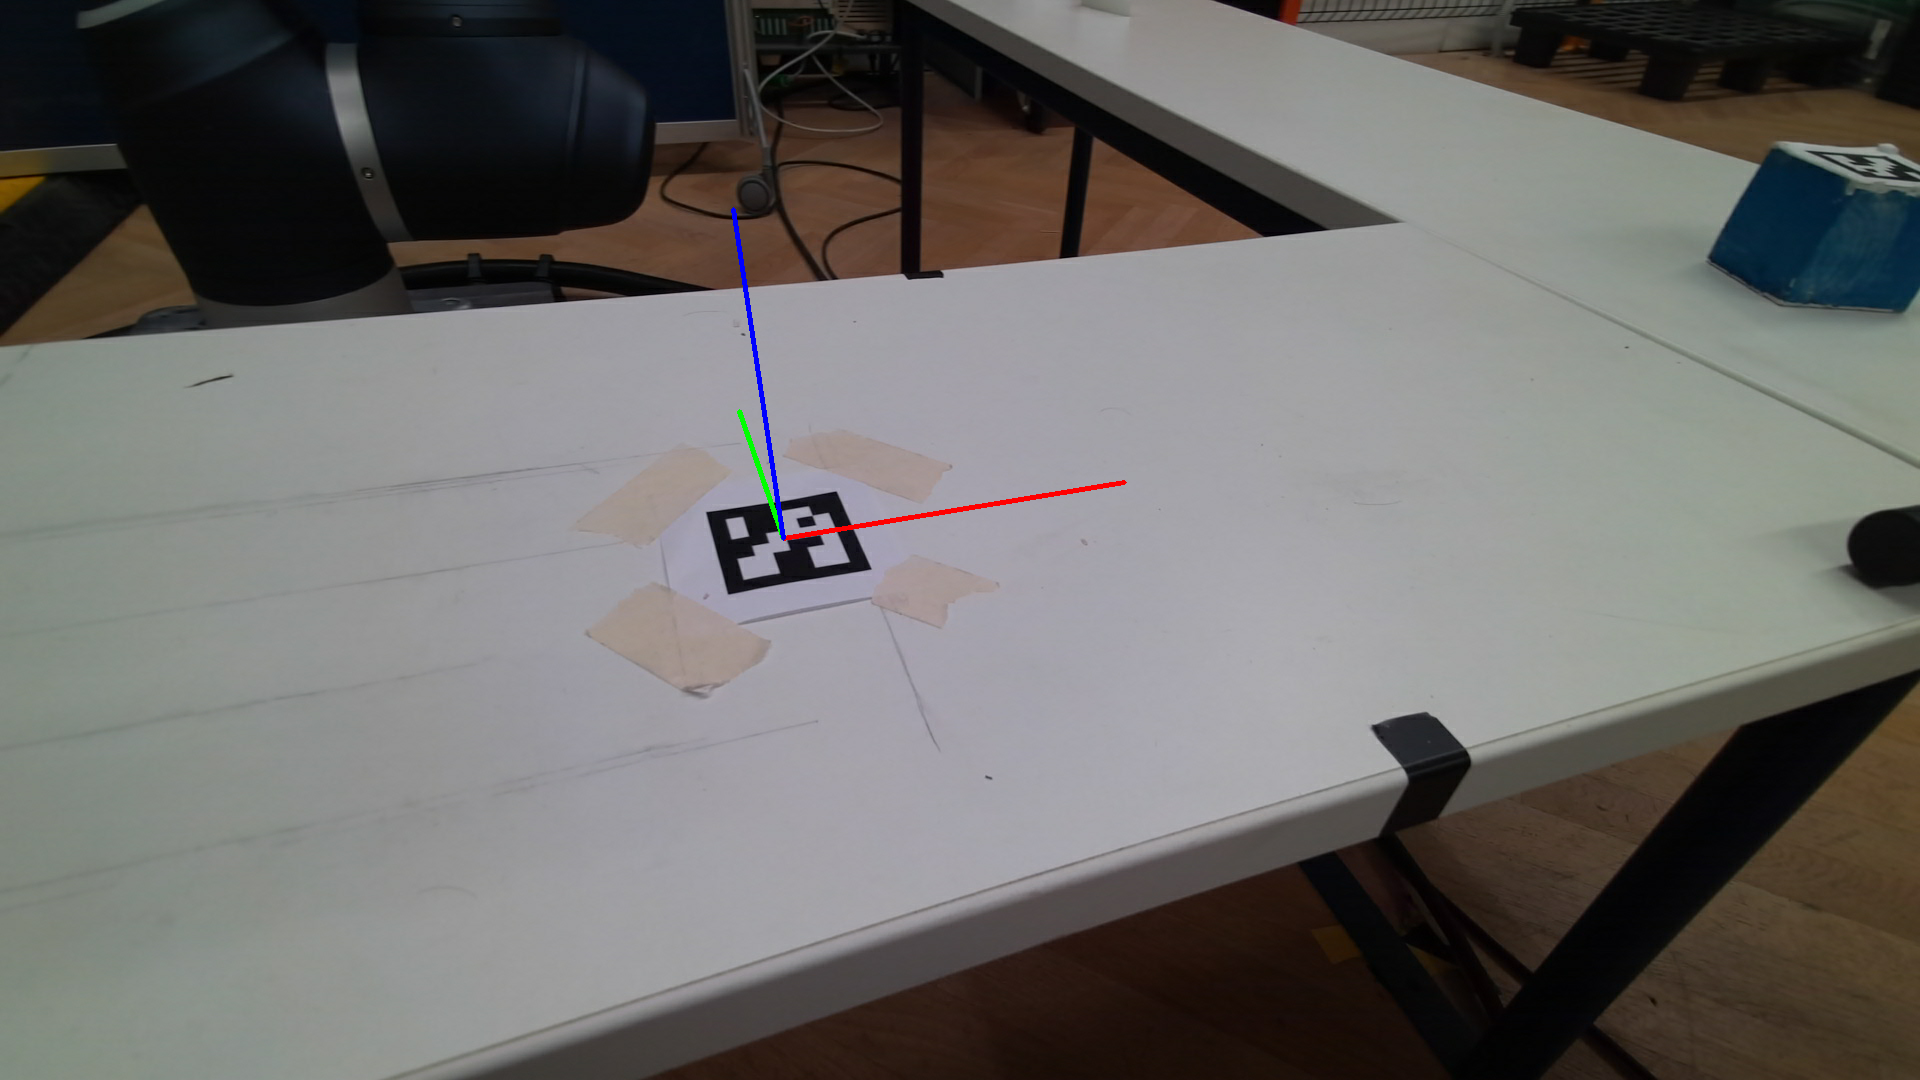
\includegraphics[width=0.8\textwidth]{output.png}
    \caption{An example of pose identification using ArUco markers.}
    \label{fig:arucoExample}
\end{figure}

Overall, non-learning based methods, while simple and computationally efficient, often require strictly controlled enviroments and specific conditions to be functional. This greatly restricts their applicability, and therefore learning-based methods are more widely used.

\section{Learning-Based Methods}
\label{s:learningbasedmethods}

Since the introduction of Convolutional Neural Networks (CNN), artifical intelligence and deep learning have been widely applied to the field of image processing, including its subfields of object detection and 6D pose estimation. The methods described in this section aim to train a CNN on vast quantities of data to perform a certain task. Based on the specifics of this task, we can categorize these approaches into three main branches: 2D-3D correspondence, direct estimation, and pose refinement. We will give a couple of examples for each of these categories.

\subsection{2D-3D Correspondence}
\label{ss:2D3D}

This class of methods uses a two step approach: they first implement a neural network to regress a set of 2-D points from an image, corresponding to a set of known feature points, and then use PnP to obtain the 6D pose of the object.

BB8\cite{BB8} uses object segmentation to perform 2D object detection, then regresses the 8 points that form the 3D bounding box of an object, but struggles with textureless symmetric or partially occluded objects. To combat these issues, PVNet\cite{PVNet} uses farthest point sampling to select keypoints on the surface of the object, and then implements a dense pixel-wise voting network, where each pixel "votes" on locations for the keypoints. RANSAC\cite{RANSAC} is then used to exclude outliers and obtain predictions with their probability distribution, which are then used for uncertainty-driven PnP.

Most approaches in this class share two common weaknesses. First, they are very perfomance-intensive when estimating the pose of multiple objects, since keypoint regression and PnP have to be computed for each object individually\cite{bukschat2020efficientpose}. Second, they are not end-to-end trainable, as the loss functions implemented do not reflect the final perfomance on the pose estimation task\cite{SS6D}. However, recent approaches have faced this issue by implementing learned or differentiable PnP algorithms, so as to enable end-to-end training\cite{EPro-Pnp}.

\subsection{Direct Estimation}
\label{ss:directestimation}

The approaches in this category exploit convolutional neural networks to directly regress the pose of an object in a single step. They are end-to-end trainable and boast better run times than the previously seen 2D-3D methods.

PoseNet\cite{PoseNet} was one of the first implementations of this concept, and was originally conceptualized for obtaining the camera pose from outdoor or indoor enviroments, and not for object pose estimation. Deep-6DPose\cite{deep6D} works by extending the Mask R-CNN\cite{Mask-R-CNN} instance segmentator, which in turn extends the Faster R-CNN\cite{Faster-R-CNN} object detector, and introduced a key technical feature by decoupling rotation and translation parameters, so as to make the pose regression loss differential. PoseCNN\cite{PoseCNN} expanded on this idea, and introduced a novel loss function that enabled it to properly handle symmetric objects.

Most networks in this category are fast and relatively accurate, but struggle in situations with partial occlusions.

\begin{table}[ht]
    \begin{center}
        \begin{tabular}{||c c c c c||} 
        \hline
        Rank & Model Name & Mean ADD & Method & Year\\ [0.5ex] 
        \hline\hline
        1 & RNNPose & 97.37 & Refinement & 2022 \\ 
        \hline
        2 & EfficientPose & 97.35 & Direct + Refinement & 2020 \\
        \hline
        3 & RePOSE & 96.1 & Refinement & 2021 \\
        \hline
        4 & EPro-PnP-6DoF v1 & 95.8 & 2D-3D & 2022\\
        \hline
        5 & ROPE & 95.61 & 2D-3D & 2021 \\
        \hline
        6 & DPOD & 95.2 & 2D-3D + Refinement & 2019\\
        \hline
        7 & HRNet  & 93.3 & 2D-3D & 2019 \\
        \hline
        8 & HybridPose & 91.3 & 2D-3D & 2020 \\
        \hline
        9 & CDPN & 89.86 & 2D-3D + Direct & 2019 \\
        \hline
        10 & PoseCNN + DeepIM & 88.6 & Direct + Refinement & 2018\\
        \hline
        \end{tabular}
    \caption{Top ten performing models on the LINEMOD dataset\cite{linemod} as of November 2022. Data taken from paperswithcode.com/sota/6d-pose-estimation-on-linemod.}
    \label{tab:top10models}
    \end{center}
\end{table}

\subsection{Pose Refinement}
\label{ss:poserefinement}

The previously explained algorithms may only give a rough estimate of the object pose at times. If greater accuracy is required, it is often necessary to use pose refinement algorithms. Approaches in this category start from an inital estimate, and then use various methods to refine it, obtaining a more accurate prediction.

DeepIM\cite{DeepIM} employs an iterative approach, by repeatedly rendering a 3D model of the object and matching it against the observed image. To ensure successive iteraterations gain in precision, it is trained not only on an annotated dataset, but also on previous outputs of the network. RNNPose\cite{RNNPose}, while also starting from a rendering and the observed image, formulates the task as a nonlinear optimization problem: it minimizes differences between correspondence fields by leveraging recent discoveries in the field of optical flow estimation, while recurrently calling itself. RNNPose currently boasts the best performance on the widely used LINEMOD\cite{linemod} dataset by a narrow margin, as highlighted by table \ref{tab:top10models}.

While refinement methods achieve remarkable performance, they have two main downsides. First, they rely on an inital estimate of the pose, so they cannot be applied independently, and second, they are relatively computationally intensive, especially when one considers that they must be run in parallel with another estimation method to generate the initial poses.

\begin{figure}[ht]
    \centering
    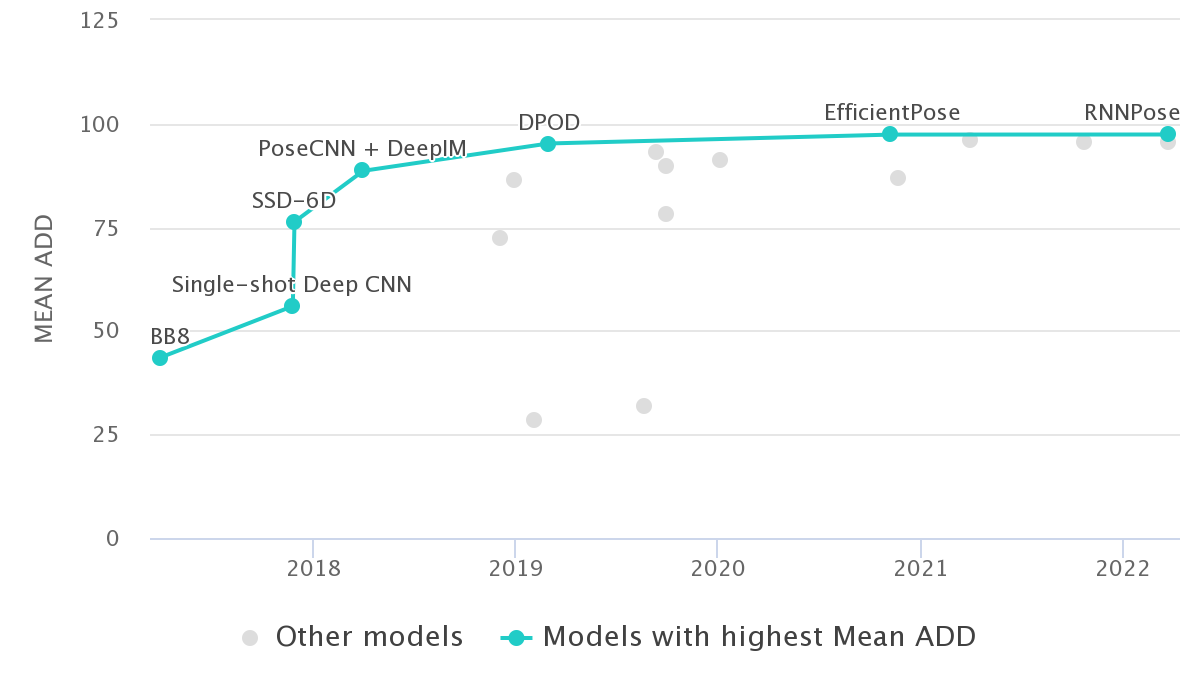
\includegraphics[width=0.7\textwidth]{linemodchart.png}
    \caption{Performance on LINEMOD of recent pose estimation algorithms by year. Graphic originates from paperswithcode.com/sota/6d-pose-estimation-on-linemod.}
    \label{fig:linemodchart}
\end{figure}

\subsection{Conclusions on Learning Approaches}

Data-driven models based on deep learning are more widely applicated than non-learning-based models, as a large variety of approaches exists, and each approach brings its own distinct advantages. When choosing a model, special attention must be given to the application the model is destined for. For single object pose estimation, especially in highly occluded enviroments, 2D-3D methods are the best choice. For multi-object pose estimation, direct estimation methods provide greater computational efficency. Whenever greater accuracy is required, pose refinement algorithms offer the best results.

\section{EfficientPose}

\begin{figure}[ht]
    \centering
    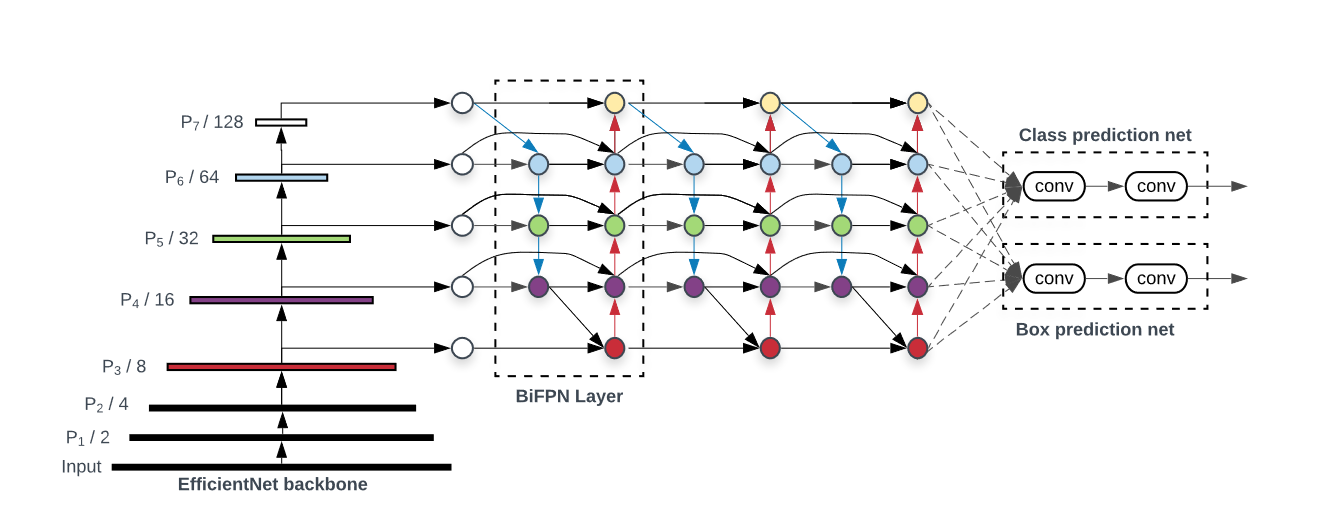
\includegraphics[width=\textwidth]{EfficientDetArchitecture.png}
    \caption{Overview of the EfficientDet architecture. BiFPN layers and subnet layers may be repeated multiple times according to resource constraints.}
\end{figure}

EfficientPose was chosen as the starting point for this thesis as it boasts state-of-the-art results while maintaining relative simplicity and low computational cost. It was designed with multi-object estimation in mind, which is especially significant, as other approaches do not scale well with the number of total detections.

Similarly to Deep-6DPose (previously mentioned in section \ref*{ss:directestimation}), it is an end-to-end direct 6D pose estimation approach that extends the functionality of a 2D network. While Deep-6D extends the segmentation network Mask-R-CNN, EfficientPose extends Google's object classification network EfficientDet\cite{EfficientDet}, which in turn builds on Google's backbone network EfficientNet\cite{EfficientNet}. We will briefly examine these two network families.

We specify "families," as both networks are based on the concept of scalability, changing network dimensions using a single hyperparameter $\phi$. For $\phi = 0$, we have a base network with minimum depth, width and resolution in an optimal ratio. By increasing the value of $\phi$, we can scale up these dimensions while mainining this ratio, thus obtaining better performance than if we had just increased the depth, width or resolution of the network individually. The results are visible in figure \ref{fig:effNetPerformance} for EfficientNet and \ref{fig:effDetPerformance} for EfficientDet: it is obvious that they both have potentially much better performance than their alternatives while maintaining significantly lower computational costs.

EfficientNet is designed using neural architecture search\cite{NAS} to provide optimal structure for the baseline, while EfficientDet expands upon this backbone by introducing a feature pyramid network\cite{FPN} (FPN). FPNs are built for multi-scale feature fusion, combining information contained in low resolution, semantically strong features with information containted in high resolution, semantically weak features. EfficientDet implements its own version of FPN, called bi-directional FPN, where top-down and bottom-up aggregation paths are then repeated a number of times dependant on the chosen $\phi$. The outputs of the Bi-FPN are then fed into two fully connected networks that perform class and bounding box prediction.

\begin{figure}[htp]
    \subfloat[EfficientNet: X values are the number of parameters used in the network, Y values are the percentage of correct answers on the Imagenet dataset\cite{imagenet}.]{%
    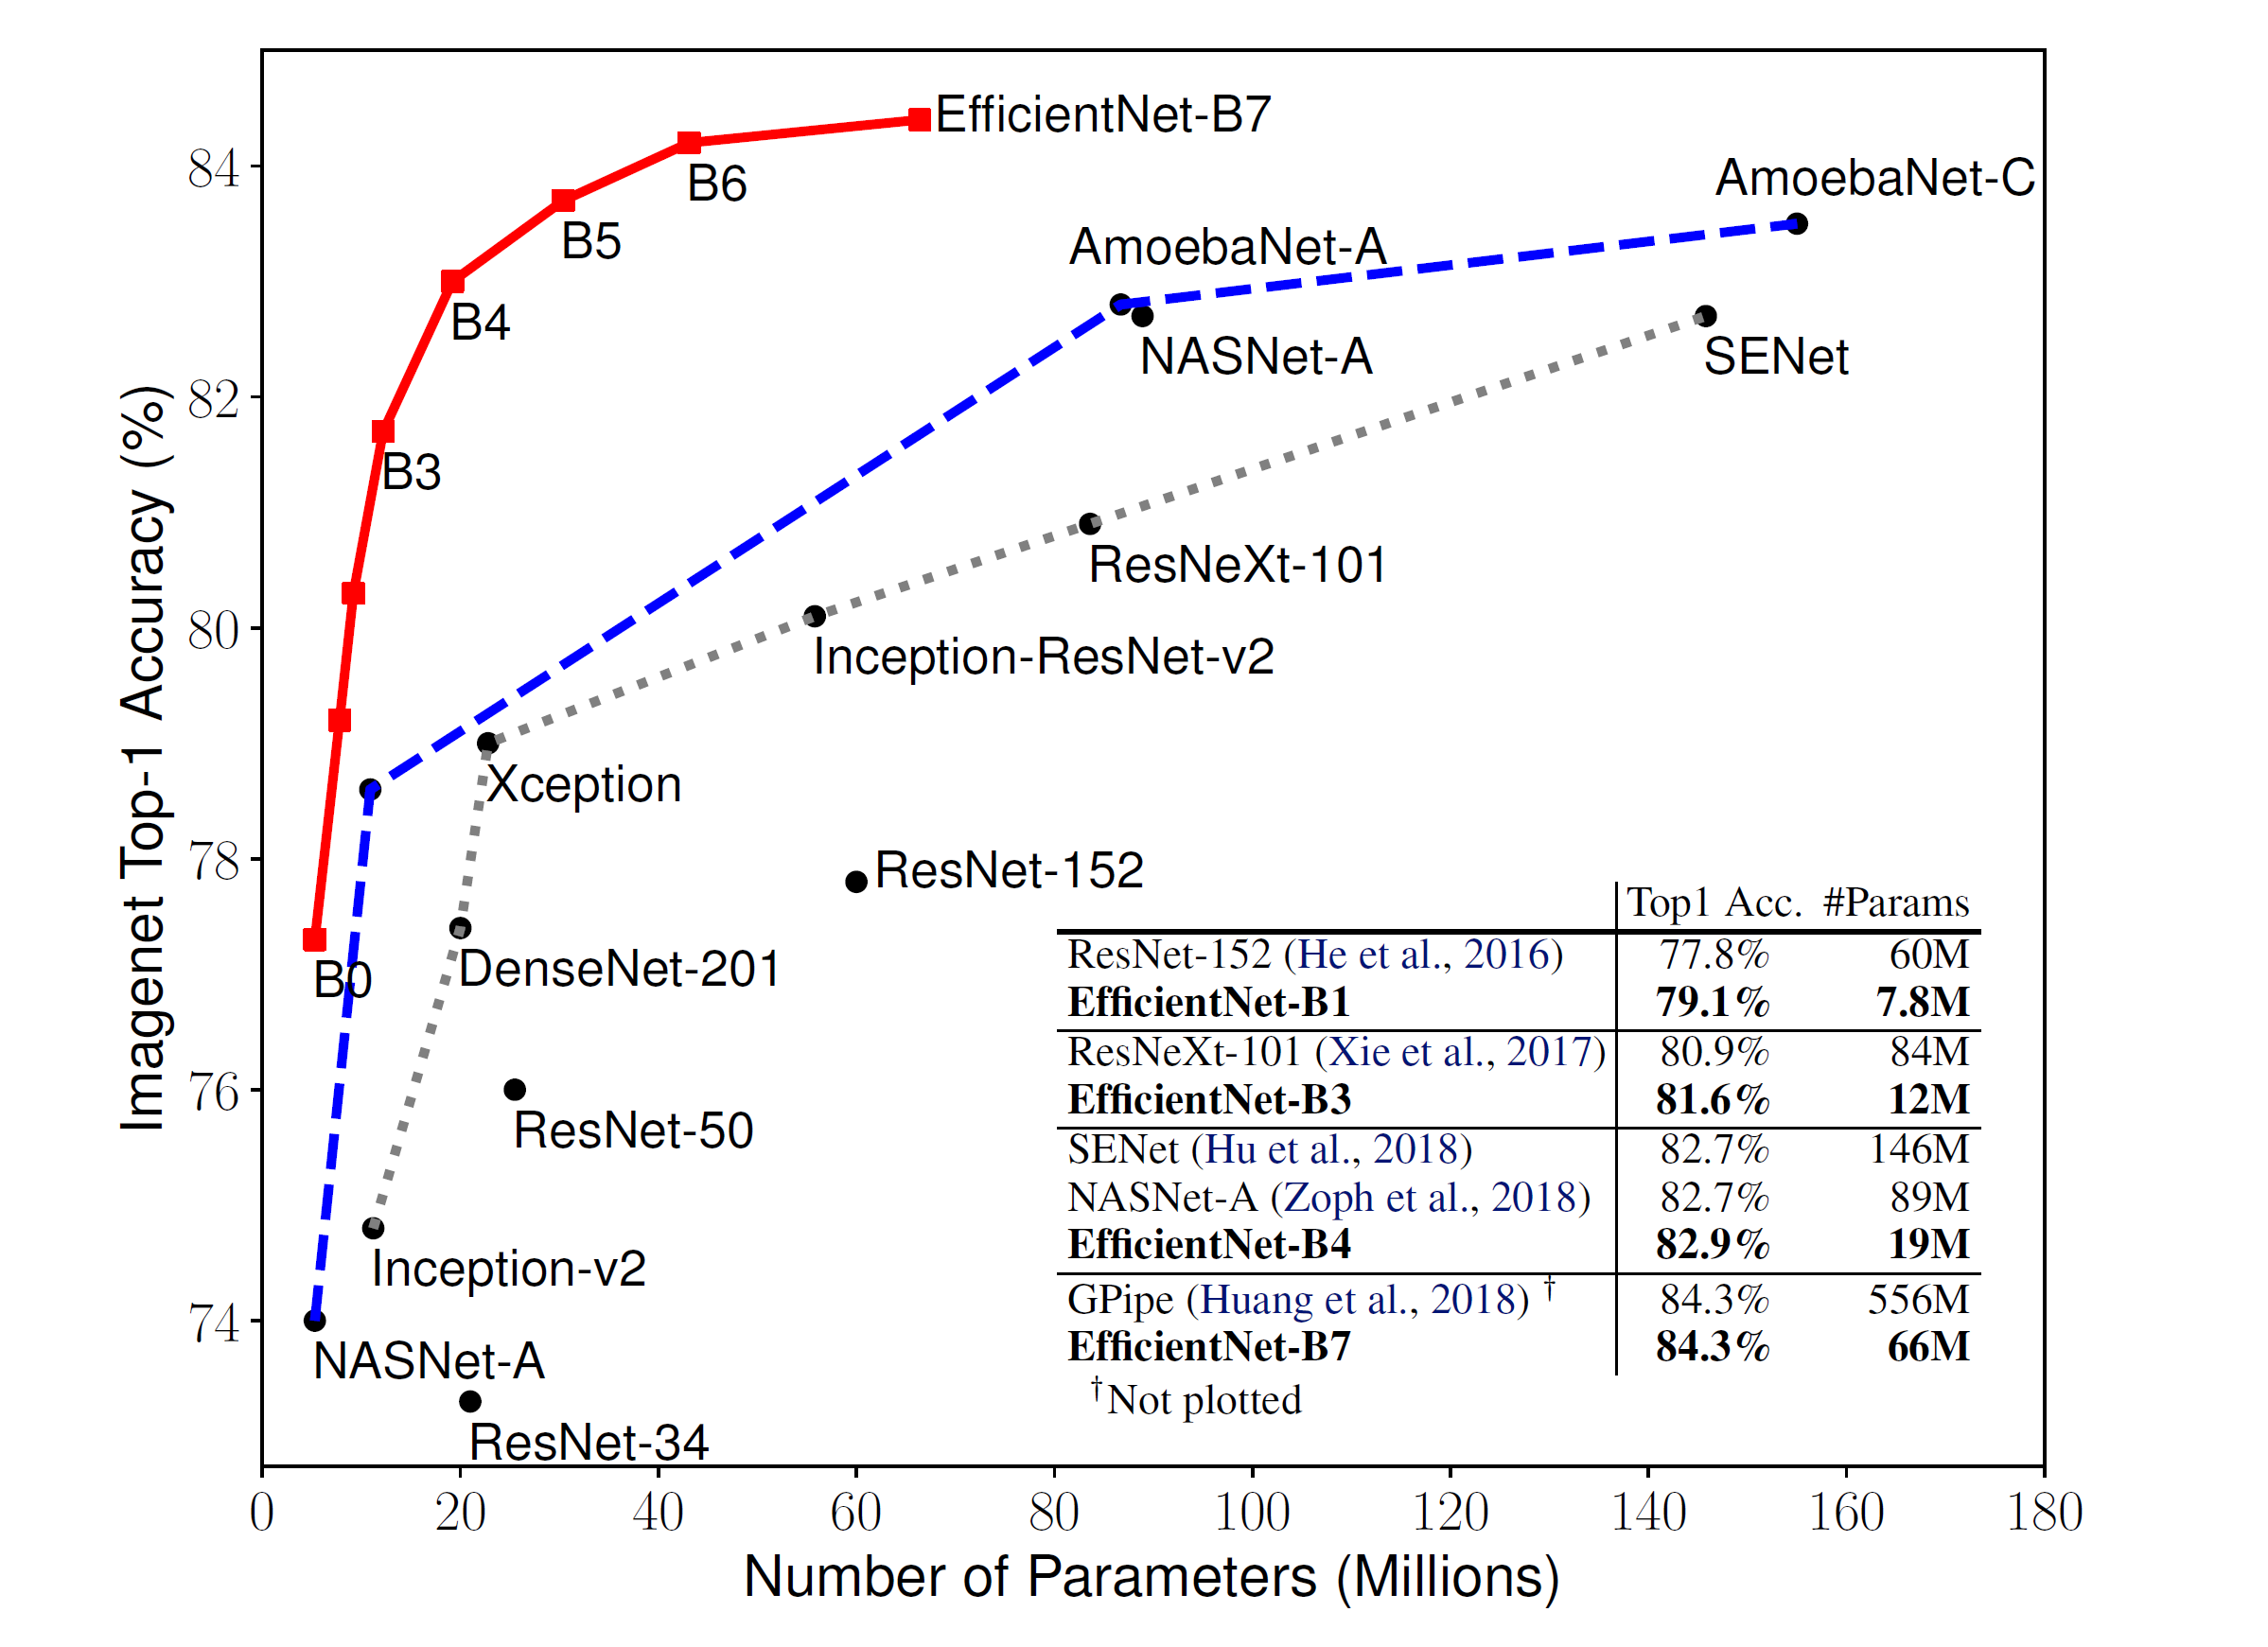
\includegraphics[width=0.7\textwidth]{EfficientNetPerformance.png}
    \label{fig:effNetPerformance}}
    
    \subfloat[EfficientDet: X values are the number of Floating Point Operations per second (FLOPs), Y values are the Average Precision (AP) tested on the Microsoft Commmon Objects in Context dataset\cite{cocodataset}.]{%
    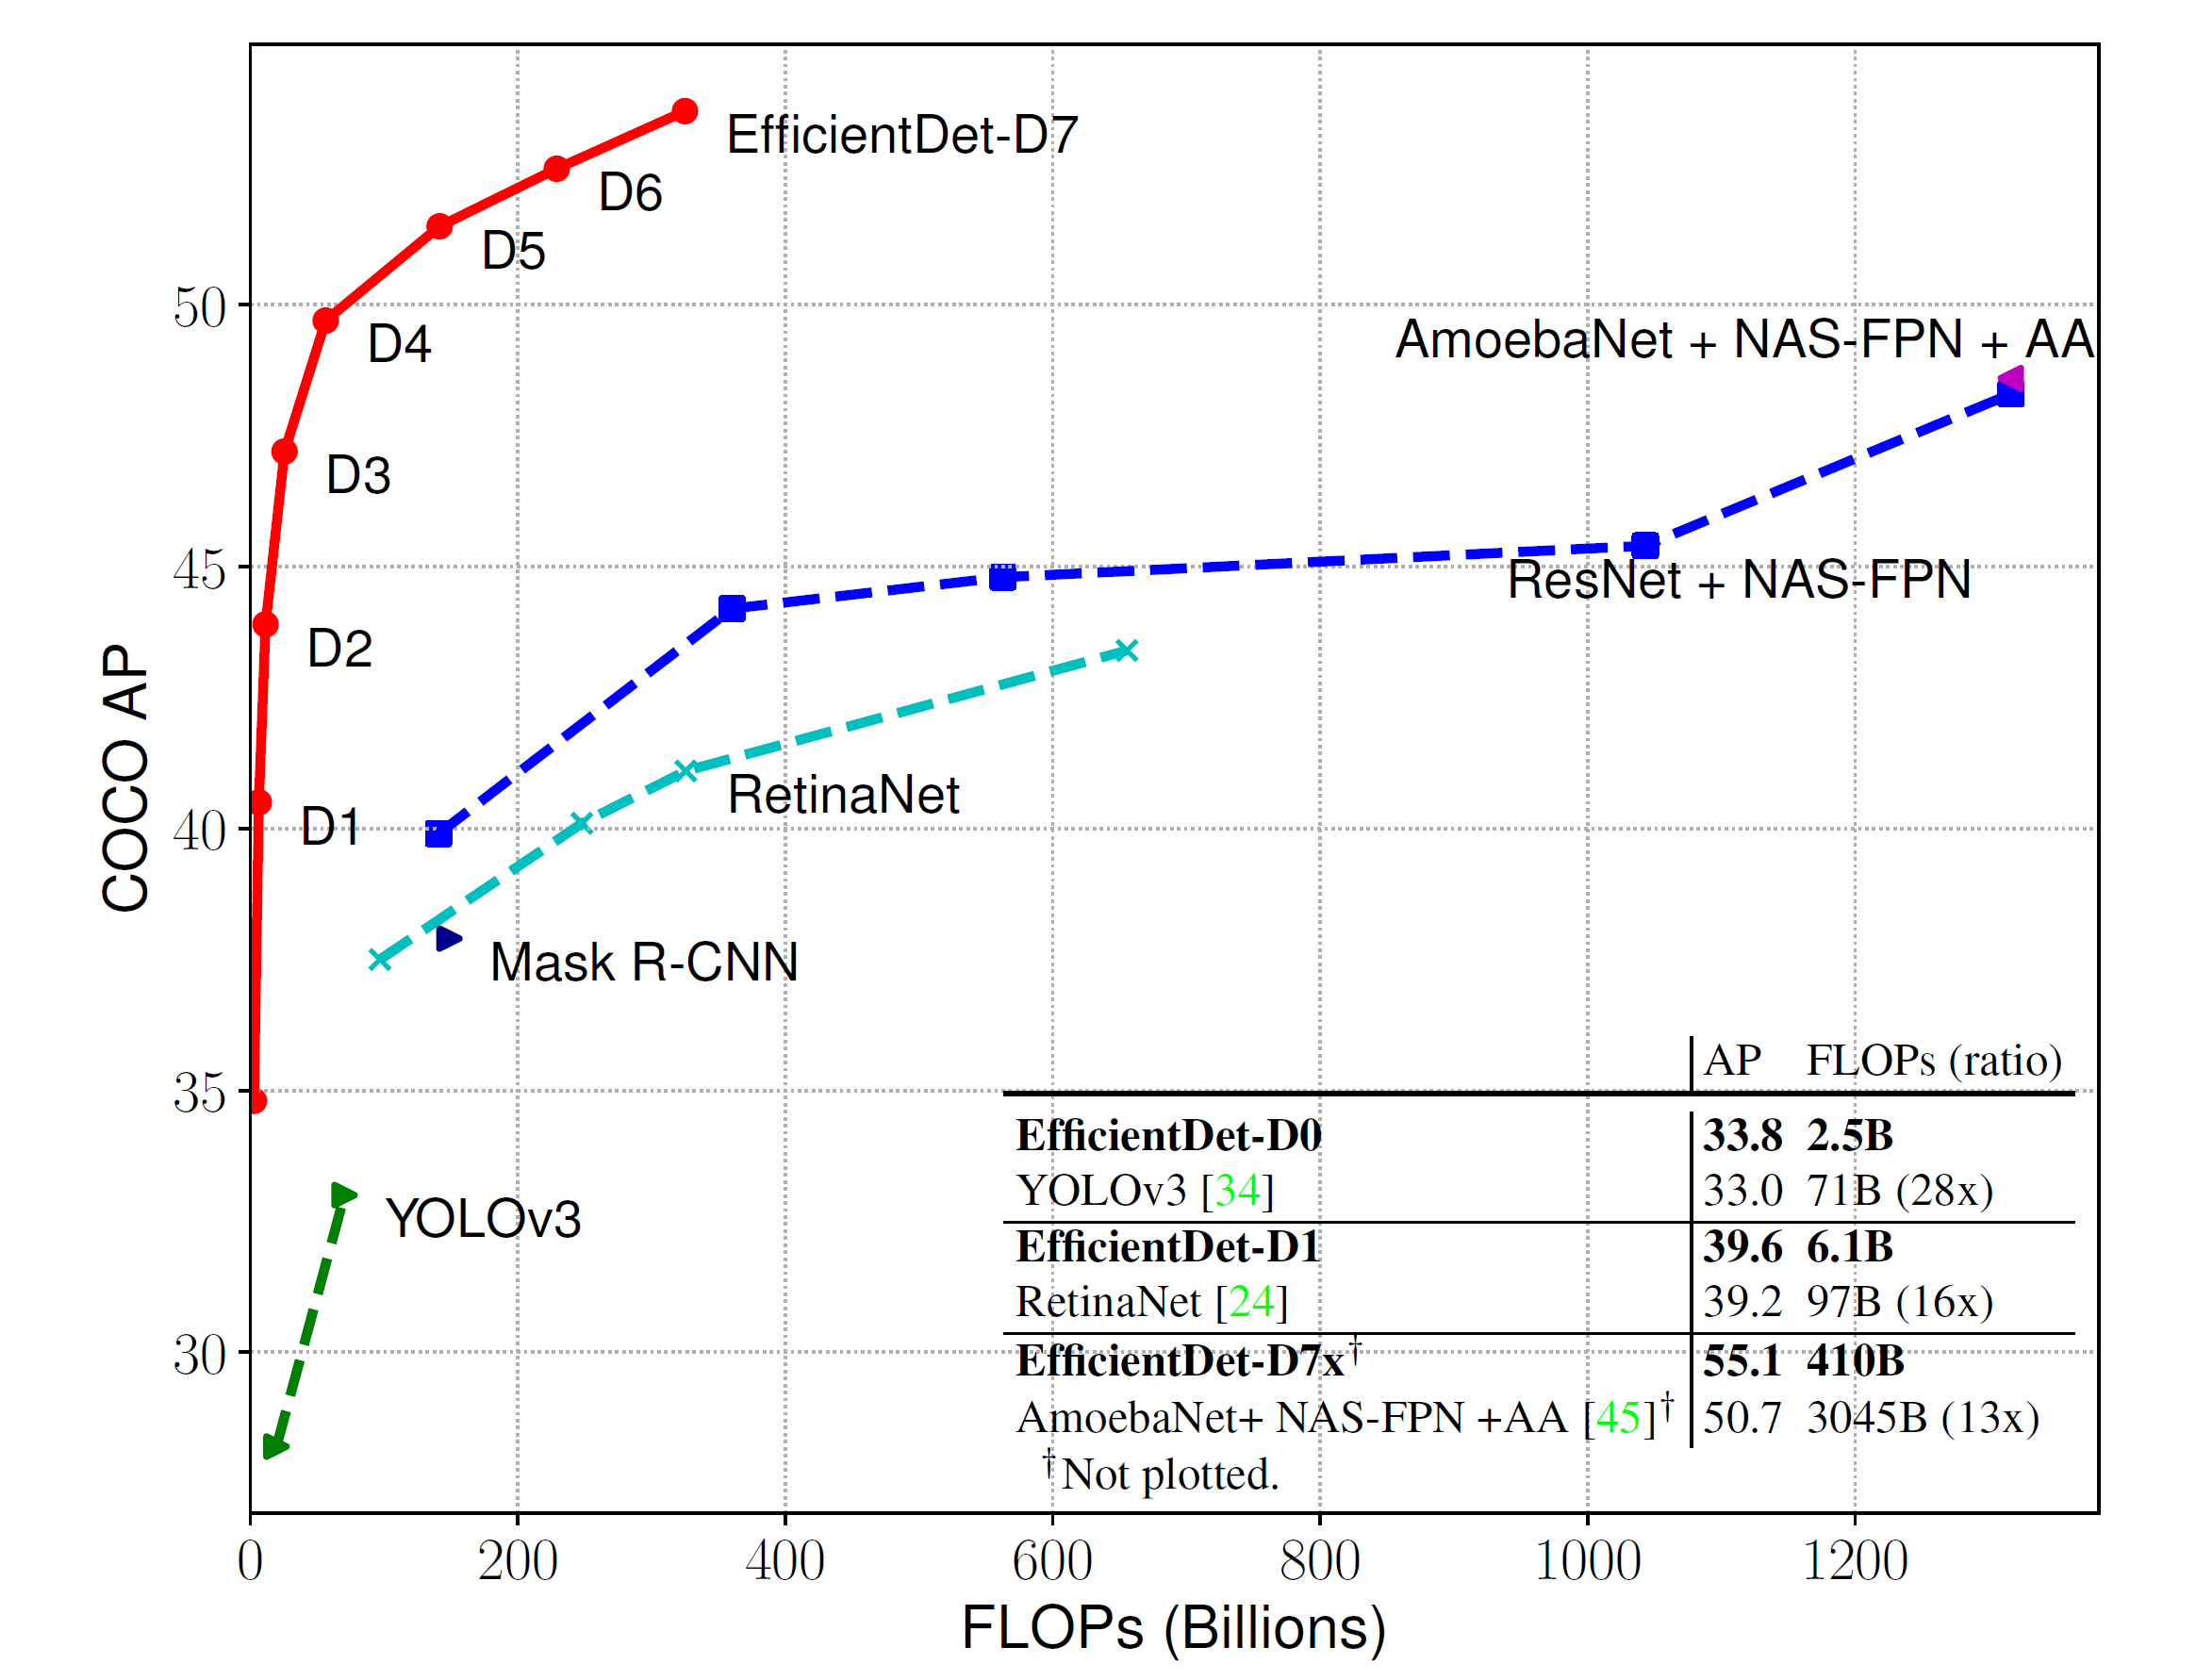
\includegraphics[width=0.7\textwidth]{EfficientDetPerformance.png}
    \label{fig:effDetPerformance}}

    \caption{Performance of the EfficientNet and EfficientDet families compared to other approaches.}
\end{figure}

The resulting network is single-shot object detector, which sets it apart from previously mentioned approaches such as Mask-R-CNN. These employ a two phase approach, with an initial region proposal step followed by the final object detection. By instead applying a single step approach, EfficientDet is much simpler and computationally efficient.

EfficientPose's expansion on this architecture is the addition of two additional subnets that predict translation and rotation, in parallel with the class and box networks. Since these networks are relatively small, additional computational costs are minimal.

The rotation network outputs a vector $R \in \mathbb{R}^3$ containing a minimal representation of the rotation, usually in Rodrigues angles, and then employs an additional iterative refinement strategy. Both the network size and the number of iterations are controlled by the hyperparameter $\phi$.

The translation network instead splits the task of predicting the position $p=[x, y, z]^T$ of the object into separate predictions of the 2D center $c = [c_x, c_y]^T$ and of the depth $z$. Then the final position $p$ can be computed using the camera intrinsic parameters by inverting the relationship:

\begin{equation}
    \begin{bmatrix}
        c_x\\c_y\\1
    \end{bmatrix}
    = \frac{1}{z}
    \begin{bmatrix}
        f_x & 0 & p_x \\
        0 & f_y & p_y \\
        0 & 0 & 1 
    \end{bmatrix}
    \begin{bmatrix}
        x\\y\\z
    \end{bmatrix}
\end{equation}

...where $f_x, f_y$ are the focal lengths and $(p_x, p_y)$ is the principal point. Thus we obtain:

\begin{equation}
    \begin{bmatrix}
        x\\y\\z
    \end{bmatrix}
    =z
    \begin{bmatrix}
        \frac{1}{f_x} & 0 & \frac{p_x}{f_x} \\
        0 & \frac{1}{f_y} & \frac{p_y}{f_y} \\
        0 & 0 & 1 \\
    \end{bmatrix}
    \begin{bmatrix}
        c_x\\c_y\\1
    \end{bmatrix}
\end{equation}

An advantage of EfficientPose's approach is that multiple class, box, rotation and translation networks for different object instances can share the same backbone and feature network. This minimizes additional computation costs for multi-object pose estimation and training, with the downside of losing accuracy compared to a network trained on a single object. 

In summary, EfficientPose is a state-of-the-art single shot 6D pose estimator which keeps the many advantages of EfficientDets, including high accuracy, scalability, and efficency, and is relatively simple to use and modify.

\section{Datasets for Pose Estimation}

Deep learning is a fundamentally data-driven approach. It aims to progressivly optimize a complicated model with tens of thousands of parameters by minimizing its loss over a large variety of training inputs; therefore these inputs are of crucial importance when trying to obtain a certain desired behaviour. They must be organized and relevant to the task, and each input, which in our case is an image, must be associated with a ground truth, which encodes the ideal result that the network should strive for. Errors or inaccuracies in the ground truth or the inputs introduce noise that could greatly influence the final results.

Thus datasets are fundamental for both training and evaluation of a pose estimation model. In this section we will examine three popular datasets used for this task: LINEMOD\cite{linemod}, Occulsion LINEMOD\cite{occlusionlinemod} and YCB-Video\cite{PoseCNN}.

\subsection{LINEMOD}
\label{ss:LINEMOD}

\begin{figure}[ht]
    \centering
    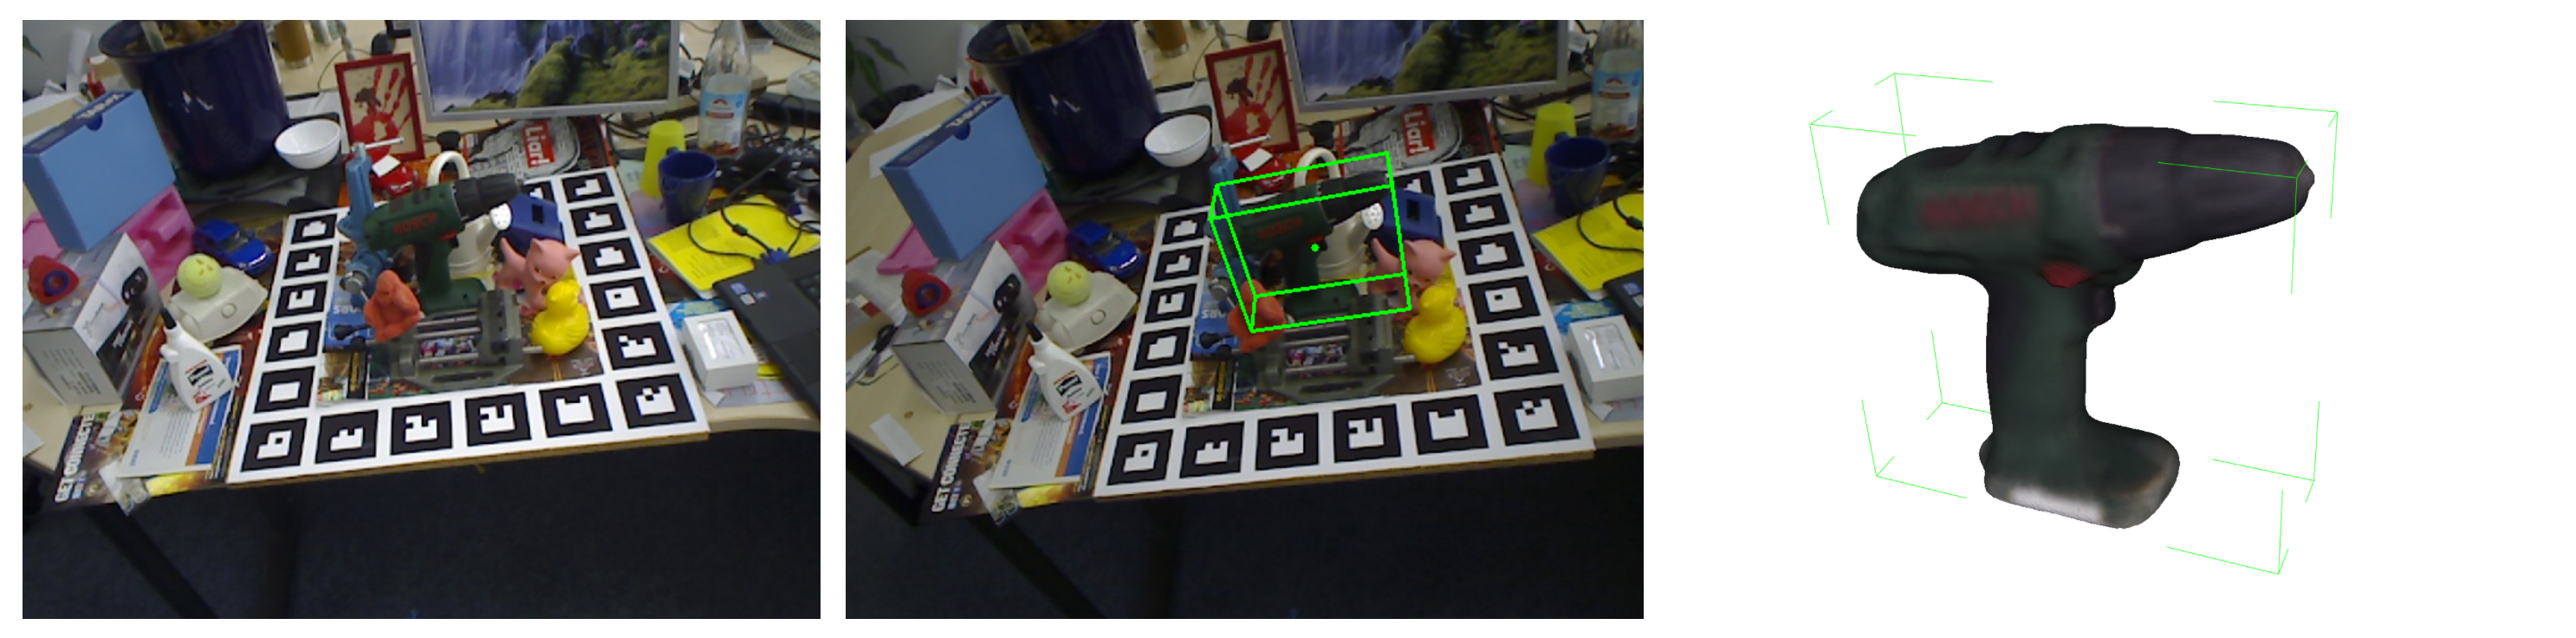
\includegraphics[width=\textwidth]{LINEMOD/LINEMOD.png}
    \caption{A basic overview of the type of data LINEMOD contains: image, ground truth and 3D model.}
    \label{fig:linemod}
\end{figure}

The LINEMOD\cite{linemod} dataset is the most popular dataset for training and evaluating 6D pose estimation methods. It is often used as a benchmark to compare different approaches.

The dataset contains images and annotations for 13 different objects, placed in 13 different cluttered scenes. For each object, around 1200 images are provided with associated ground truths, including separate rotations and translations. Furthermore, for each object a colored 3D model is provided. The dataset also contains depth images corresponding to each scene, but since our network only takes RGB input, we are not interested in these.

LINEMOD was generated by sticking the tracked objects to the center of a board surrounded by markers. Since the position of each object on the board is known, and the marker pose relative to the camera can be easily and robustly estimated as described in section \ref{s:notlearningbasedmethods}, the final pose of the object can be computed with excellent accuracy. Furthermore, since the images were taken in a uniformly divided hemispherical space around the center board, each object has images comprising a good distribution of poses from multiple orientations.

\subsection{Occlusion LINEMOD}

Occlusion LINEMOD\cite{occlusionlinemod} is a multi-object pose estimation dataset that builds on a subset of LINEMOD; in particual it only uses images from one scene. It differs from the base dataset in two aspects: first, all 13 objects are annotated in every scene, and second, objects often present heavy occlusion due to clutter and positioning. This makes it extremely challenging when compared to vanilla LINEMOD.

Occlusion has been used mainly to train RGB-D models, but some pure RGB approaches \cite{PVNet}\cite{PoseCNN} have also used it as a test dataset, while employing LINEMOD for training. EfficientPose, being a multiple object detection network, employs Occlusion for both training and testing one of its models.

\subsection{YCB-Video}

\begin{figure}[ht]
    \centering
    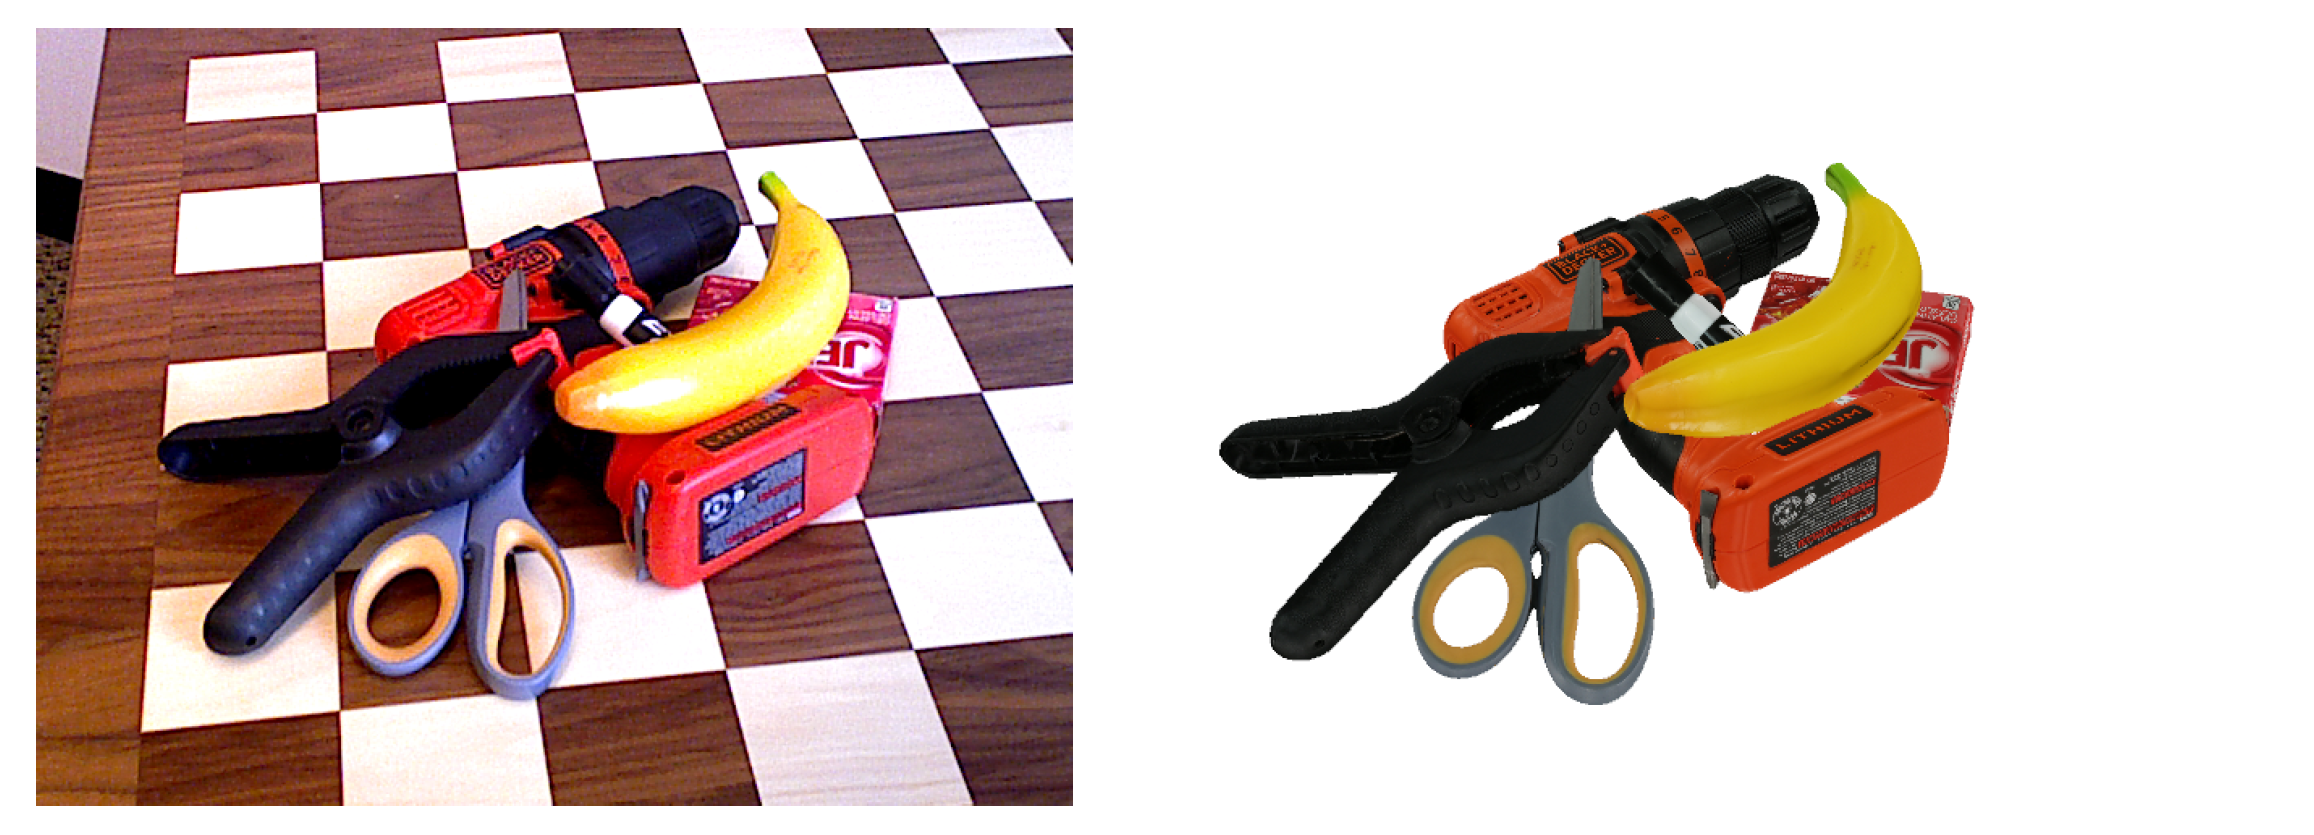
\includegraphics[width=0.8\textwidth]{YCBVideo.png}
    \caption{An example image from YCB-Video, with a rendering of the 3D object models positioned according to its annotations. Image taken from \cite{PoseCNN}.}
\end{figure}

The YCB-Video dataset\cite{PoseCNN}, while less popular than LINEMOD, addresses one of the latter's critical weaknesses: its very low data count for each object, when compared to typical datasets for deep learning.

YCB-Video consists of 92 videos for a total of 133,827 frames, containing 21 objects from the YCB Object and Model Set\cite{YCBSet}. In the first frame of each video, object poses are refined using depth information, thus presenting an accurate initial pose. The camera trajectory is then inferred for the other frames from the depth video, and finally both the trajectory and poses are further refined in a global optimization step. This makes for efficient and fast data acquisition, resulting in a dataset that is two orders of magnitute greater than LINEMOD while maintaining similar precision.